%%%% CAPÍTULO 3 - MATERIAL E MÉTODOS (PODE SER OUTRO TÍTULO DE ACORDO COM O TRABALHO REALIZADO)
%%
%% Deve apresentar o modelo utilizado, a modelagem
%% empregada, as simplificações necessárias, a
%% metodologia e a descrição do método de cálculo 
%% utilizado no desenvolvimento da pesquisa para que
%% a mesma possa ser reconstituída. Deve ainda 
%% apresentar resultados de amostras e comentários.
%% Deve apresentar a descrição da montagem 
%% experimental, metodologia para a obtenção de 
%% resultados, análise de erros, amostra de resultados
%% obtidos e comentários. Atenção: Esta parte pode ser
%% subdividida em mais capítulos de acordo com a 
%% especificidade do assunto.

%% Título e rótulo de capítulo (rótulos não devem conter caracteres especiais, acentuados ou cedilha)
\chapter{Material e Métodos}\label{cap:materialemetodos}

\section{Transporte Coletivo na Cidade de Curitiba}

\definecolor{clauciane}{RGB}{204, 0 ,0}

\definecolor{courb2020}{RGB}{0, 204 ,0}

Segundo o Instituto de Pesquisa e Planejamento Urbano de Curitiba (IPPUC), o sistema de transporte coletivo de Curitiba é composto por linhas urbanas e metropolitanas. Estas linhas são caracterizadas quanto a sua função e categoria, sendo diferenciadas por cores, conforme ilustra a Figura ~\ref{fig:linhas}. 

Segue uma breve descrição de cada linha ofertada~\cite{Cur:19}:

\begin{itemize}
    \item Expresso Ligeirão: Linhas operadas por veículos biarticulados nas cores azul e vermelha com capacidade para 250 passageiros. Caracterizada por deslocamentos mais rápidos em canaletas exclusivas e número reduzido de paradas, os embarques e desembarques do Expresso Ligeirão são realizados em terminais e estações-tubo. 

    \item Expresso: São linhas operadas por veículos tipo biarticulados, na cor vermelha, com capacidade para até 170 passageiros. As linhas Expresso ligam os terminais de integração ao centro da cidade, através das canaletas exclusivas. Embarques e desembarques são feitos em nível nos terminais e nas estações-tubo existentes no trajeto.

    \item Linha Direta (Ligeirinho): Linhas operadas com veículos nas cores prata ou cinza.  Os veículos operantes nas linhas diretas realizam com paradas em média a cada 3 km, com embarque e desembarque em nível nas estações-tubo. As linhas diretas são linhas complementares, principalmente das linhas expressas e interbairros.

    \item Interbairros: São linhas que ligam os diversos bairros e terminais sem passar pelo Centro da cidade. Operadas por veículos tipo padron ou articulados, na cor verde.
    
    \item Alimentador: São operadas por veículos tipo micro, comum ou articulados, nas cores laranja ou amarela. As linhas alimentadoras são responsáveis pela conexão dos terminais de integração aos bairros de cada região.

    \item Troncal: As linhas troncais ligam os terminais de integração ao Centro da cidade, utilizando vias compartilhadas. Operam com veículos tipo padron ou articulados, nas cores amarela ou laranja. 

    \item Convencional: Sem a realização de integração, as linhas convencionais ligam os bairros ao Centro da cidade. Operam com veículos tipo micro ou comum, nas cores amarela ou laranja.
        
    \item Circular Centro:  A linha circular centro atende os principais pontos atrativos da região central de Curitiba, tais como praças, shoppings, Rodoviária e Biblioteca Pública. É operada com veículos tipo micro-ônibus e apresenta tarifa diferenciada.

    \item Linha Turismo: Linha caracterizada pela realização do trajeto de turismo urbano de Curitiba. Passa pelos principais parques e pontos turísticos da cidade (tarifa diferenciada). Com saída do Centro, os ônibus da linha turismo são to tipo double deck e são da cor verde claro.

\end{itemize}

 \begin{figure}[!h]
 \caption{Composição da frota}
     \centering
     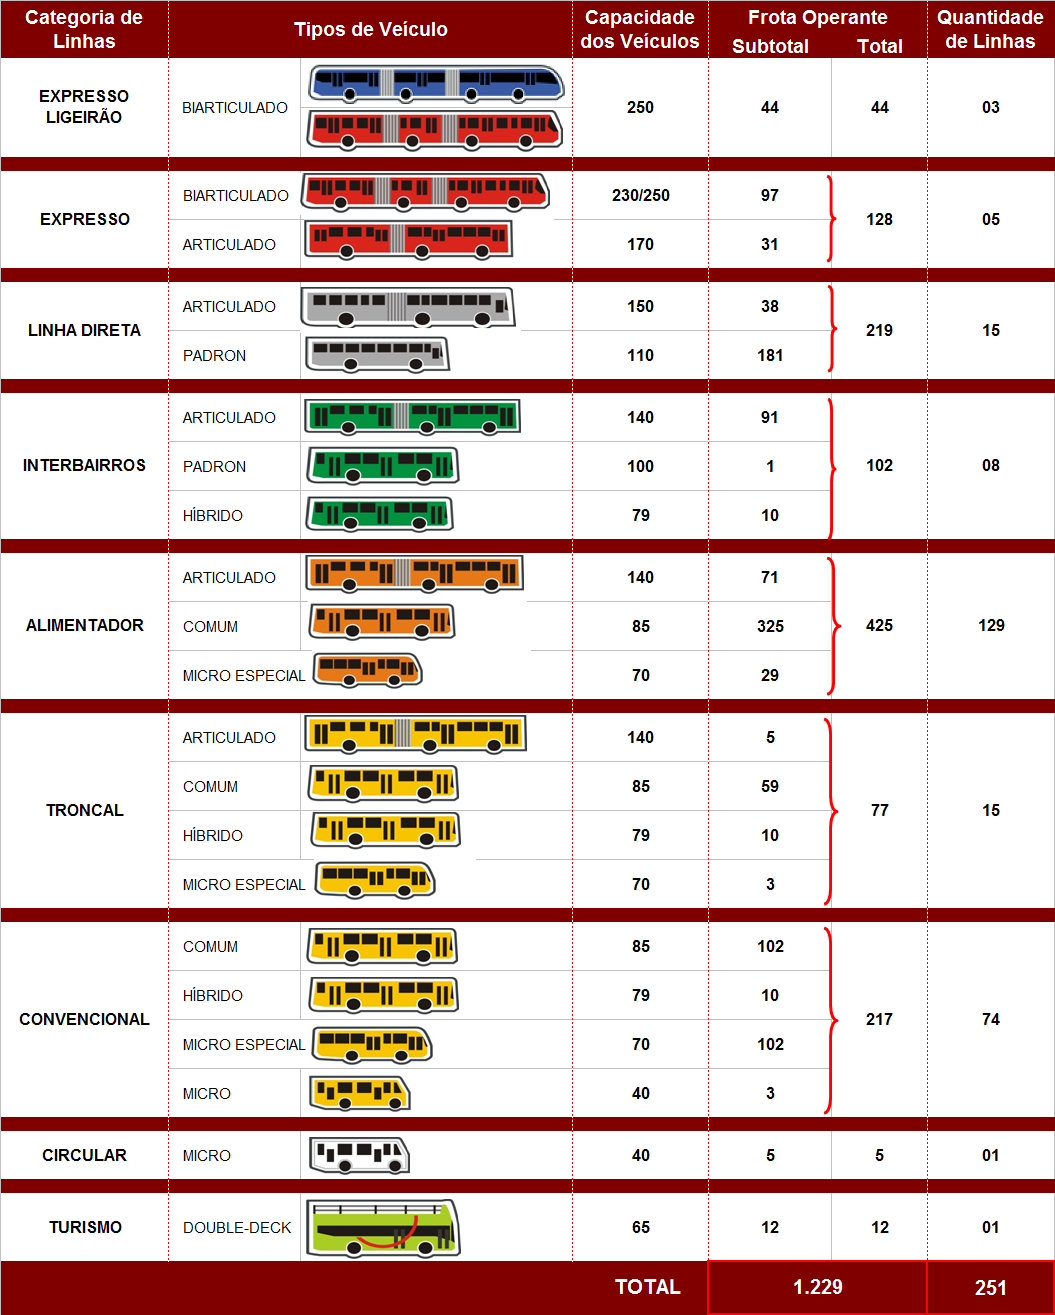
\includegraphics[scale=.40]{./Capitulo3/img/composicao-frota.png}
         \label{fig:linhas}
     \fonte{Rede Integrada de Transporte~\cite{Cur:19}}
 \end{figure}


Os terminais, assim como as linhas do transporte público são divididas em categorias e  recebem uma classificação sendo divididos em: terminais de ponta, terminais intermediários, terminais de bairros, terminais de área central e terminais metropolitanos. Tal divisão, como o nome sugere, indica a posição dos mesmos no sistema de transporte, conforme ilustra a Figura ~\ref{fig:terminais}.
 \begin{figure}[!h]
 \caption{Localização e classificação dos terminais de ônibus de Curitiba}
     \centering
     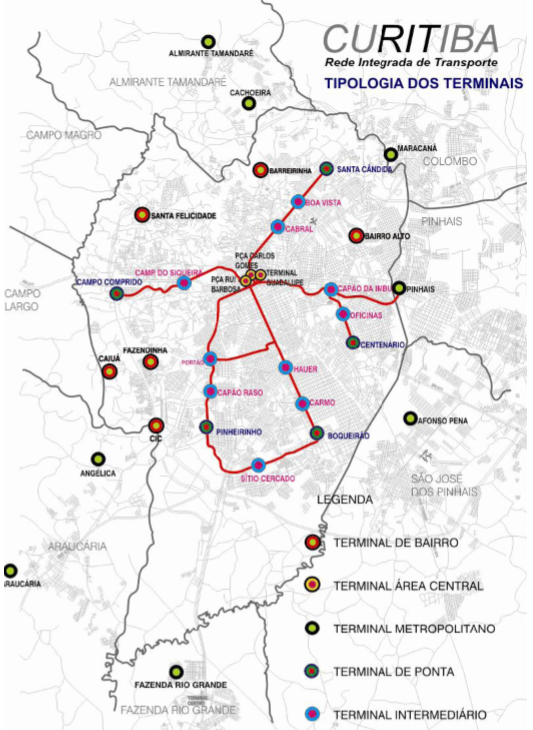
\includegraphics[scale=.95]{./Capitulo3/img/terminais.png}
         \label{fig:terminais}
     \fonte{Plano de Mobilidade Urbana de Curitiba, IPUCC 2019}
 \end{figure}

\section{Modelo Proposto} \label{sec:met}


O modelo proposto para o transporte público de Curitiba é mostrado na Figura~\ref{fig:model}. Este modelo tem por base o modelo de~\cite{wach:19}.

A Figura~\ref{fig:model} apresenta um grafo com vértices temporais (\emph{Line} e \emph{Trip} ) e espaço-temporais (\emph{BusStop} e \emph{Event}). Os vértices temporais carregam informações que variam com o tempo, enquanto os vértices espaço-temporais possuem informações de tempo associadas a dados de posicionamento georreferenciado. Vértices adicionais definem propriedades estáticas inerentes à operação de transporte público de Curitiba(\emph{Timetable}, \emph{ServiceCategory}, \emph{Color}, \emph{BusStopType} e \emph{Neighbourhood}), assim como agrupamentos temporais do modelo que permitem recuperar informações para diferentes escalas de tempo (\emph{Year}, \emph{Month}, \emph{Day} e \emph{Hour}). Em resumo, o modelo da Figura~\ref{fig:model} representa dependências temporais e espaço-temporais entre os vértices do grafo que descreve a operação de um sistema de transporte.

 \begin{figure}[!h]
 \caption{Modelo TVG da movimentação dos ônibus do transporte.}
     \centering
     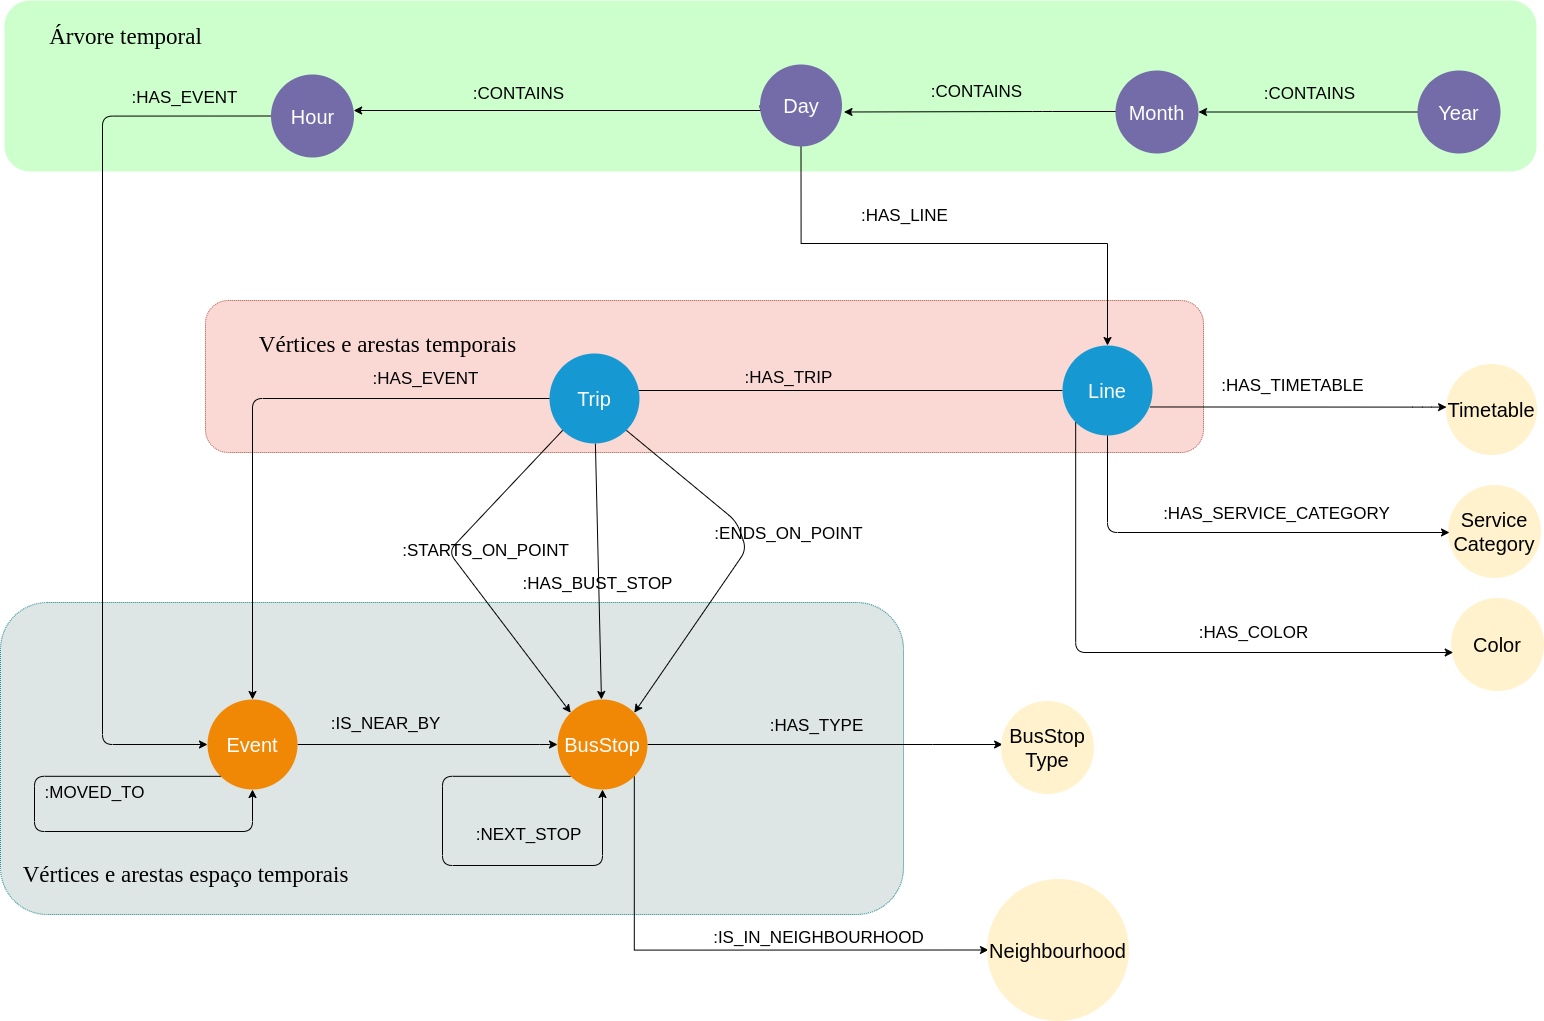
\includegraphics[scale=.25]{./Capitulo3/img/graph-model.png}
         \label{fig:model}
     \fonte{Autoria própria}
 \end{figure}
 
 

Os atributos dos vértices do grafo da Figura~\ref{fig:model} são mostrados nas Tabelas~\ref{tab:vertice_line}, \ref{tab:vertice_trip}, \ref{tab:vertice_busstop}, \ref{tab:vertice_event}, \ref{tab:vertice_color}, \ref{tab:vertice_service_category}, \ref{tab:vertice_busstop_type},\ref{tab:vertice_timetable} e \ref{tab:vertice_neighbourhood}. 

Cada linha de ônibus (vértices \emph{Line} - Tabela~\ref{tab:vertice_line}) dá origem a viagens (vértices \emph{Trip} - Tabela~\ref{tab:vertice_trip}).

As viagens são programadas (vértices \emph{Timetable} - Tabela~\ref{tab:vertice_timetable}) para serem executadas por veículos, que geram sequências de movimentação e paradas (vértices \emph{Event} - Tabela~\ref{tab:vertice_event}). Estas paradas incluem paradas nos pontos de ônibus (vértices \emph{BusStop} - Tabela~\ref{tab:vertice_busstop}) para embarque e desembarque de passageiros. Além disso, as viagens possuem pontos de ônibus inicial, intermédiario(s) e final (vértices \emph{BusStop} - Tabela~\ref{tab:vertice_busstop}). Além disso, linhas de ônibus podem ser agrupadas e recuperados por dia (aresta \texttt{HAS\_LINE}), assim como eventos podem ser agrupados e recuperados por hora (aresta \texttt{HAS\_EVENT}). Os atributos das arestas da Figura~\ref{fig:model} são mostrados na Tabela~\ref{tab:arestas} do Apêndice. As arestas estabelecem relacionamentos entre os vértices do grafo, além de carregarem atributos espaciais, temporais ou espaço-temporais para orientar consultas futuras.
Conforme será discutido na Seção~\ref{sec:impl}, a construção do grafo correspondente ao modelo da Figura~\ref{fig:model} no Neo4j é realizada a partir dos dados brutos da operação do transporte.


\subsection{Vértices}

Os vértices em roxo (\emph{year}, \emph{month}, \emph{day} e \emph{hour}) representam elementos essencialmente temporais representados. Tais elementos constituem a árvore temporal do grafo.

Já os vértices em azul representam elementos temporais relacionados ao modelo de transporte, sendo constituído pelos vértices \emph{Line} - Tabela~\ref{tab:vertice_line} e \emph{Trip} - Tabela ~\ref{tab:vertice_trip}:
 
\begin{table}[!htb]
    \caption{Atributos dos vértices \emph{Line}: identificam a linha de ônibus.}
    \label{tab:vertice_line}
    \centering
    \footnotesize
    \begin{tabular}{p{2.5cm}p{6cm}} 
    \hline
    Atributo & Descrição\\
    \hline
    \texttt{line\_name}        & nome da linha \\
    \texttt{card\_only}        & indicador se a linha aceita somente cartão \\
    \texttt{line\_code}        & código da linha \\
    \hline
    \end{tabular}
\end{table}


\begin{table}[htb]
    \caption{Atributos dos vértices \emph{Trip}: identificam os sentidos das linhas.}
    \label{tab:vertice_trip}
    \centering
    \footnotesize
    \begin{tabular}{p{2.5cm}p{2.5cm}}
        \hline
        Atributo & Descrição\\
        \hline
        \texttt{line\_way} & sentido da linha \\
        \hline  
    \end{tabular}
\end{table}


Vértices em laranja identificam elementos espaço-temporais na rede, isto é, que possuem atributos de geolocalização assim como relações temporais. No modelo são destacados os vértices \emph{BusStop} - Tabela ~\ref{tab:vertice_busstop} e \emph{Event} - Tabela~\ref{tab:vertice_event} :

\begin{table}[!htb]
    \caption{Atributos dos vértices \emph{BusStop}:  identificam os pontos de ônibus.}
    \label{tab:vertice_busstop}
    \centering
    \footnotesize
    \begin{tabular}{p{2.5cm}p{5cm}} 
        \hline
        Atributo & Descrição\\
        \hline
        \texttt{name} & nome do ponto de ônibus  \\
        \texttt{number} & número do ponto de ônibus \\
        \texttt{neighborhood\_code} & identificador único do bairro onde o ponto de ônibus está localizado\\
        \texttt{h3\_index10} & georreferenciamento h3 do ponto de ônibus  \\
        \texttt{latitude} & latitude do ponto \\
        \texttt{longitude} & longitude do ponto \\
        \hline
    \end{tabular}
\end{table}


\begin{table}[!htb]
    \caption{Atributos dos vértices \emph{Event}: identificam eventos de posicionamento dos ônibus.}
    \label{tab:vertice_event}
    \centering
    \footnotesize
    \begin{tabular}{p{3cm}p{6cm}} 
        \hline
        Atributo & Descrição\\
        \hline
        \texttt{moving\_status} & tipo do evento. [STOPPED, MOVING] \\
        \texttt{avg\_velocity} & velocidade do evento em km/h \\
        \texttt{event\_timestamp} & \emph{timestamp} do evento de parada do ônibus  \\
        \texttt{latitude} & latitude da parada  \\
        \texttt{longitude} & longitude da parada  \\
        \texttt{vehicle} & identificador único do veículo \\
        \hline  
    \end{tabular}
\end{table}

Vértices em amarelo identificam definem propriedades estáticas inerentes à operação de transporte público de Curitiba. Estes são constituídos pelos vértices \emph{Timetable} - Tabela~\ref{tab:vertice_timetable}, \emph{ServiceCategory} - Tabela~\ref{tab:vertice_service_category}, \emph{Color}- Tabela~\ref{tab:vertice_color}, \emph{BusStopType}- Tabela~\ref{tab:vertice_busstop_type} e \emph{Neighbourhood})- Tabela~\ref{tab:vertice_neighbourhood}.
 

\begin{table}[htb]
    \caption{Atributos dos vértices \emph{Timetable}: identificam os horários programados das linhas.}
    \label{tab:vertice_timetable}
    \centering
    \footnotesize
    \begin{tabular}{p{2.5cm}p{6.5cm}}
        \hline
        Atributo & Descrição\\
        \hline
        \texttt{start\_time} & horário programado para o inicio da viagem \\
        \texttt{end\_time} & horário programado para o término da viagem \\
        \texttt{line\_way} & sentido da viagem \\
        \texttt{start\_point} & ponto de ônibus onde a viagem se inicia \\
        \texttt{end\_point} & ponto de ônibus onde a viagem termina \\
        \texttt{timetable} & número da tabela de agendamento de horários \\
        \hline  
    \end{tabular}
\end{table}

\begin{table}[htb]
    \caption{Atributos dos vértices \emph{ServiceCategory}: identificam as categorias de serviço das linhas.}
    \label{tab:vertice_service_category}
    \centering
    \footnotesize
    \begin{tabular}{p{2.5cm}p{6.5cm}}
        \hline
        Atributo & Descrição\\
        \hline
        \texttt{value} & nome da categoria de serviço da linha \\
        \hline  
    \end{tabular}
\end{table}

\begin{table}[htb]
    \caption{Atributos dos vértices \emph{Color}: identificam as cores das linhas.}
    \label{tab:vertice_color}
    \centering
    \footnotesize
    \begin{tabular}{p{2.5cm}p{6.5cm}}
        \hline
        Atributo & Descrição\\
        \hline
        \texttt{value} & nome da cor \\
        \hline  
    \end{tabular}
\end{table}

\begin{table}[htb]
    \caption{Atributos dos vértices \emph{BusStopType}: identificam as tipos de pontos de ônibus.}
    \label{tab:vertice_busstop_type}
    \centering
    \footnotesize
    \begin{tabular}{p{2.5cm}p{6.5cm}}
        \hline
        Atributo & Descrição\\
        \hline
        \texttt{value} & nome do tipo de ponto de ônibus \\
        \hline  
    \end{tabular}
\end{table}

\begin{table}[htb]
    \caption{Atributos dos vértices \emph{Neighbourhood}: identificam os bairros da cidade de Curitiba.}
    \label{tab:vertice_neighbourhood}
    \centering
    \footnotesize
    \begin{tabular}{p{2.5cm}p{2.5cm}}
        \hline
        Atributo & Descrição\\
        \hline
        \texttt{name} & nome do bairro \\
        \texttt{code} & identificador único do bairro \\
        \texttt{section\_name} & nome da regional \\
        \texttt{section\_code} & código da regional \\
        \texttt{h3\_index10} & georreferenciamento h3 do bairro \\
        \hline  
    \end{tabular}
\end{table}


\subsection{Arestas}

As arestas conectam dois vértices de um grafo. Elas e seus atributos são descritos na Tabela~\ref{tab:arestas}.

\begin{table}[!htb]
    \caption{Descrição das arestas: significado das conexões e atributos.}
    \label{tab:arestas}
    \centering
    \small
    \begin{tabular}{ p{5cm}p{8.5cm}} 
    \hline
    Rótulo & Descrição\\
    \hline
    \texttt{IS\_NEAR\_BY}            & conecta o ônibus a paradas (veloc. $< 15$ km/h)\\
    \texttt{STARTS\_ON\_POINT}       & Conecta um sentido de linha a seu ponto de ônibus inicial determinando o início de seu roteiro. \\
    \texttt{HAS\_BUST\_STOP}         & Identifica os pontos de ônibus que compõe um sentido da linha\\
    \texttt{ENDS\_ON\_POINT}         & Conecta um sentido de linha a seu ponto de ônibus final determinando o término de seu roteiro. \\
    \texttt{HAS\_COLOR}              & conecta a linha a sua cor \\ 
    \texttt{HAS\_TYPE}               & conecta o ponto de ônibus ao seu tipo \\ 
    \texttt{HAS\_SERVICE\_CATEGORY}  & conecta a linha a sua categoria de serviço \\ 
    \texttt{IS\_IN\_NEIGHBOURHOOD}   & conecta o ponto de ônibus ao bairro em que está localizado \\ 
    \texttt{HAS\_TIMETABLE}          & conecta a linha à sua programação horária \\ 
    \texttt{HAS\_TRIP}               &  Uma linha pode ter diversos sentidos: logo, esta aresta realiza a conexão da linha com os sentidos da linha. \\ 
    \texttt{HAS\_LINE}               & Conecta a árvore temporal a existência da linha operante. Uma linha pode deixar de operar ao longo do tempo. \\ 
    \texttt{HAS\_EVENT}              & agrupa as informações de eventos do veículo por hora\\
    \hline
    \multirow{4}{*}{\texttt{NEXT\_STOP}} & conecta pontos de ônibus consecutivos da viagem: \\
    & \texttt{line\_code}: Código da linha\\
    & \texttt{line\_way}: Sentido da linha\\
    & \texttt{distance}: Distância em metros entre dois pontos de ônibus \\
    & \texttt{line\_name}: Nome da linha\\
    \hline
    \multirow{4}{*}{\texttt{MOVED\_TO}}           & Liga a sequência de eventos de um determinado veículo. \\
    & \texttt{delta\_time\_in\_sec}: Tempo em segundos entre dois eventos.\\
    \hline
    \end{tabular}
\end{table}



\section{Métricas de Redes Complexas} \label{sec:metr}


Uma vez que o grafo do sistema de transporte descrito na seção anterior é modelado e armazenado no Neo4j, métricas de redes complexas podem ser computadas para avaliar o comportamento do sistema. 
Tais métricas permitem uma avaliação da importância dos vértices na rede (pontos de ônibus), tanto do ponto de vista estático da topologia da rede quanto dinâmico da movimentação dos ônibus, e sua relação com os outros pontos da rede.
Esta seção descreve as métricas utilizadas neste trabalho: 

\subsection{Centralidade de grau}


Proposto por~\cite{free:79}, a {\bf centralidade de grau} é proporcional ao número de arestas (de entrada, ou de saída em grafos direcionados) que se conectam a um determinado vértice. Quanto maior a centralidade de grau de um vértice, maior é o número de conexões com outros vértices.

No caso da rede de transporte, na perspectiva de dinamicidade da rede através da interatividade de veículos com seus respectivos pontos de ônibus, a centralidade de grau de um vértice \emph{BusStop} é proporcional ao número de paradas de ônibus no respectivo ponto. Isso pode significar que pontos com elevada centralidade de grau podem corresponder a locais de potencial congestionamento ou de formação de comboios decorrente de uma estratégia de atendimento de demanda elevada. 

Na perspectiva da rede estática, isto é, isolando-se somente os pontos de ônibus e suas conexões, a centralidade de grau de um vértice \emph{BusStop} é proporcional ao número de linhas de ônibus que passam pelo vértice, já que apenas arestas para outros vértices \emph{BusStop} são consideradas. Um ponto ponto de ônibus com grande número de conexões apresenta uma grande oferta de linhas.

\subsection{Centralidade de intermediação}


Introduzido por \cite{free:77} como uma medida para quantificar o controle de um ser humano sobre a comunicação entre outros seres humanos em uma rede social, a {\bf centralidade de intermediação} (\emph{betweenness centrality}) quantifica quão importante um vértice (ou uma aresta) é na definição dos caminhos possíveis entre vários (ou todos) os pares de vértices de uma rede. Isso permite calcular qual a capacidade da rede se ``recuperar'' em caso de remoção de um ou mais vértices. Também é importante, pois auxilia na identificação de vértices que atuam como ``intermediários de serviços'' na rede.

Em outras palavras, a remoção de vértices com elevada centralidade de intermediação podem degradar ou mesmo interromper o fluxo de informação em uma rede. 

Para um vértice, a centralidade de intermediação é definida pela proporção dos caminhos que empregam um determinado vértice em relação a todos os caminhos existentes, ou seja:

 \begin{equation}
     B(u) = \sum_{s \neq u \neq t }^{} p(u) / p,
 \end{equation} 
na qual:

 \begin{itemize}
 \item $u$: é um vértice.
 \item $p$: é o número total de caminhos entre os vértices $s$ e $t$.
 \item $p(u)$: é o número de caminhos entre os vértices $s$ e $t$ que passam pelo vértice $u$.
\end{itemize}  

No contexto de sistemas de transporte, vértices com significativo $B$ são potenciais pontos de estrangulamento do sistema, dada a dependência que os caminhos possíveis desse sistema têm desse vértice. Essa dependência pode ser temporal (ocorre em um intervalo de tempo específico) ou espacial (depende da posição espacial do ponto de ônibus), de acordo com o contexto de análise.

\subsection{Page rank}


O {\bf \emph{page rank}} foi concebido com o intuito de ranquear páginas (\emph{web sites}) relevantes da \emph{World Wide Web}. 

Usando o conceito presente em cadeias de Markov e/ou difusão em redes complexas, pode-se determinar os vértices mais significativos do ponto de vista de fluxos existentes em uma rede, quando o regime estacionário é atingido. Pode-se traduzir esse regime estacionário como a tendência de um usuário aleatório sempre chegar em uma determinada página, ou os dados em redes de comunicação sempre trafegarem por um determinado roteador.

A ideia é que o fluxo de navegação dos usuários defina a relevância das páginas ao reforçar suas interconexões (\emph{hyperlinks}). O algoritmo PageRank \cite{brin:98} traduz a ideia intuitiva de que usuários em geral tendem a acessar páginas e navegar pela WWW usando \emph{hiperlinks} até uma certa profundidade. Assim, páginas bem posicionadas no fluxo de navegação são relevantes, pois tendem a ser muito visitadas pelos usuários. 
No contexto das redes de transporte, um ponto de ônibus com elevado \emph{page rank} pode indicar conexões com outros pontos importantes. Por exemplo, ligações diretas entre terminais de ônibus no caso estático.


\subsection{Caminho mínimo}

O {\bf caminho mínimo} entre dois vértices é o caminho com o menor número de arestas, no caso de arestas não ponderadas. 
Define-se caminho entre dois vértices quaisquer como a sequência de vértices, ligados dois a dois por arestas, que deve ser percorrida para conectá-los. As arestas podem ser ponderadas ou não, definindo características das ligações entre dois vértice e afetando a definição do caminho. A partir dos caminhos existentes entre dois nós quaisquer, define-se como caminho mais curto aquele cujo ``esforço'' exigido para percorrê-lo é o menor dentre os caminhos existentes.

Caso as arestas sejam ponderadas, deve-se considerar a soma dos pesos das arestas do caminho de um vértice a outro. A determinação de caminhos mínimos (considerando todos os pares de vértices de uma rede) é informação significativa para o planejamento urbano e a operação de um sistema de transporte, pois pode induzir no fluxo de pessoas na cidade. Algoritmos de caminho mínimo identificam rotas de conexão entre dois pontos da cidade de forma a minimizar o tempo de percurso necessário no transporte público \cite{Mart:2009, Larson:81}. Uma vez conhecidos os caminhos mínimos de todos os vértices para todos os outros da rede, define-se o {\bf diâmetro da rede} como o caminho mínimo mais longo da rede.

% \subsection{Conectividade}

% \textcolor{courb2020}{
% Conectividade é um propriedade que indica existe pelo menos um caminho entre todos os pares de vértices de uma rede. Caso não haja, existem sub-grafos isolados dentro da rede.
% No contexto das redes TVGs aplicadas ao sistema de transporte público, a evolução temporal desse sistema pode ou não gerar intervalos de tempo nos quais parte da rede perde conectividade com o restante da rede. Essa mudança na conectividade da rede pode ser um comportamento estrutural (ou seja, é um fenômeno recorrente da rede) ou uma anomalia (um fenômeno aleatório, como um acidente que bloqueie a passagem de veículos por uma via pública).
% }

\subsection{Diâmetro e densidade de rede}

A partir do resultado do cálculo de caminhos e caminhos mínimos pode ser identificado o diâmetro (geodésico) de uma rede. O diâmetro de uma rede é o caminho mínimo mais longo dessa rede, ou seja, a distância entre dois vértices cujo caminho mínimo é o mais longo a ser percorrido. 

Naturalmente, o contexto de análise pode implicar que o diâmetro possa ser calculado a partir de atributos dos vértices e/ou arestas, como tempo exigido para percorrer dada par de vértice conectado, ou a distância entre esses pares de vértices conectados.
A densidade da rede mede a similaridade entre a rede e um grafo completo (grafo em que há um aresta para todos os seus pares de vértices) e pode ser definida como:

 \begin{equation}
     D = \mid E \mid / \mid N \mid ( \mid N \mid -1),
 \end{equation} 
na qual:

 \begin{itemize}
 \item $N$: é o número total de vértices.
 \item $E$: é o número total de arestas.
\end{itemize}  


\section{Plataforma Computacional} \label{sec:impl}

A plataforma computacional desenvolvida gera um banco de dados de grafo no Neo4j a partir do \emph{dataset} disponibilizado pela operação do transporte coletivo de Curitiba.


\subsection{Dataset}

\textcolor{courb2020}{
O portal de dados abertos de Curitiba fornece diariamente um \emph{dataset} em formato JSON (JavaScript Object Notation) com informações sobre o transporte coletivo da cidade. Conforme mencionado anteriormente, o transporte opera em média com uma frota de 1.410 ônibus que atende cerca de 1.389.731 passageiros por dia com 251 linhas de ônibus, 329 estações e 21 terminais.
}

\textcolor{courb2020}{
A empresa URBS (gestora da Rede Integrada de Transporte Coletivo de Curitiba) define um conjunto de tabelas que contêm informações referentes às linhas de ônibus existentes, seus pontos de parada (que podem atender múltiplas linhas), os itinerários das linhas, os veículos que percorrem essas linhas, o percurso georeferenciado das linhas e o relacionamento entre essas informações. A descrição destas tabelas pode ser encontrada no dicionário de dados disponível no repositório de dados abertos. 
}
%\peix{Tais informações também estão disponíveis em forma de web service e pode ser acessado mediante a solicitação de login e senha. O dicionário de dados contendo a descrição das informações disponibilizadas pode ser obtido em \cite{dadosabertos}}

\textcolor{courb2020}{
Parte destes dados, que alimentam o fluxo de transformações descrito na Seção~\ref{subsec:work}, são detalhados nas Tabelas~\ref{tab:linhas}, \ref{tab:pontos_linha}, \ref{tab:tabela_veiculo} e \ref{tab:veiculos} do Apêndice.
}

%\ric{Seria importante caracterizar também a dimensão desta base. Por exemplo, para 1 mês de captura de dados, estamos falando de qual volume de dados? Mostrar em uma tabela: número de linhas, viagens, ônibus, etc?}


% \ric{A Tabela~\ref{tab:data} mostra estatísticas do \emph{dataset} utilizado, com informações sobre o transporte coletivo de Curitiba coletados durante um mês de operação.}

% \begin{table}[h]
%     \caption{Estatísticas do \emph{dataset} do transporte de Curitiba para 1 mês de operação \mar{(qual mês/ano?)}.}
%     \label{tab:data}
%     \centering
%     \begin{tabular}{ccccc} 
%         \hline
%         No. de registros? &No. de linhas &No. de pontos &No. de ônibus &No. de viagens\\
%         \hline
%         xxx &xxx &xxx &xxx &xxx \\
%         \hline  
%     \end{tabular}
% \end{table}

%\ric{É IMPORTANTE? É importante salientar que essas tabelas apresentam redundâncias de dados, pois não foram normalizadas segundo preceitos de banco de dados. Isso significa que foi necessário pré-processá-lo para identificar e remover inconsistências.}

\subsection{Python}


Criada na década de 1980 por Guido van Rossum na Holanda, Python é uma linguagem de programação multifuncional de alto nível que é usada em um ampla gama de domínios e campos técnicos~\cite{Yves:2018}.

Python é uma linguagem de programação interpretada, orientada a objetos e de alto nível, com tipagem dinâmica, o que o torna muito atraente para o desenvolvimento rápido de aplicativos, assim como para uso como uma linguagem de \emph{script} com a finalidade de conectar componentes existentes.
Sua sintaxe é simples e de fácil aprendizado enfatizando a legibilidade e manutenibilidade de código. Python suporta módulos e pacotes, incentivando assim a modularização de programas e reutilização de código.
 
Atualmente, a linguagem Python é amplamente utilizada, desde universidades nas mais diversas áreas científicas, até grandes corporações e instituições financeiras.

Segue algumas das principais características da linguagem Python:

\begin{itemize}

\item \emph{Open source}: Python e a maioria das bibliotecas e ferramentas de suporte disponíveis são
open source e geralmente vêm com licenças bastante flexíveis e abertas.

\item Interpretada: Python utiliza um interpretador denominado CPyhon que traduz o código fonte em tempo de execução para código \emph{byte code} executável.

\item Multi paradigma: Python suporta diferentes paradigmas de programação como orientação a objetos, funcional ou programação procedimental.

\item Multi propósito: Python pode ser utilizado para desenvolvimento de código rápido e interativo, bem como para construir grandes aplicações.

\item \emph{Cross-platform}: Python está disponível nos mais conhecidos sistemas operacionais, tais como, \emph{Windows}, \emph{Linux} e \emph{MacOS} e pode ser utilizado para o desenvolvimento de aplicações \emph{Desktop}, assim como aplicações \emph{Web}. Além disso Python pode ser utilizado em grandes conjuntos de \emph{clusters} e servidores potentes, assim como em pequenos dispositivos como \emph{Raspberry Pi}.

\item Dinamicamente tipada: Tipos de dados em Python são inferidos em tempo de execução e não previamente declarados como na maioria das linguagens de programação compiladas. 

\item Indentação ciente: Em contraste com a maioria das outras linguagens de programação, Python usa indentação para marcar blocos de código em vez de parênteses, colchetes ou ponto e vírgula.

\item \emph{Garbage collector}: Python possui \emph{garbage collection} automatizado, o que evita a necessidade do gerenciamento de memória pelo programador.

\end{itemize}


\subsection{Neo4J}

Neo4J (\emph{Network Exploration and Optimization 4 Java}) é um sistema gerenciador de banco de dados não relacional, orientado à grafos, desenvolvido pela empresa Neo Technology. É implementado em Java e acessível por programas escritos em outras linguagens utilizando \emph{Cypher Query Language} através de um \emph{endpoint} HTTP ou através de um protocolo denominado \emph{bolt}.
Neo4J é open-source em sua versão "community edition" e está disponível através de uma licença  GPLv3 (General Public License) para a versão Community Edition, e AGPLv3 (Affero General Public License) para versão Enterprise Edition.

O banco de dados Neo4j implementa um tipo de grafo denominado \emph{property graph model}, capaz de representar multigrafos direcionados, rotulados e com atributos. Estes grafos permitem a representação de vértices e arestas rotulados, além de metadados (propriedades) associados aos vértices e arestas~\cite{rod:10}, particularmente importantes na implementação de TVGs. Além disso, o banco de dados Neo4j tem outras características que favorecem a implementação: (i) armazenamento persistente e transacional de grafos de elevada dimensão; suporte para análise em profundidade via buscas eficientes de múltiplos saltos; (iii) suporte para linguagem declarativa de \emph{queries} de grafos denominada Cypher\footnote{https://neo4j.com/docs/cypher-manual/current/}.


This graph data model gives us four different fundamental building blocks to
structure and store our data. Let's go through them:


 \begin{figure}[!h]
 \caption{Property Graph Model}
     \centering
     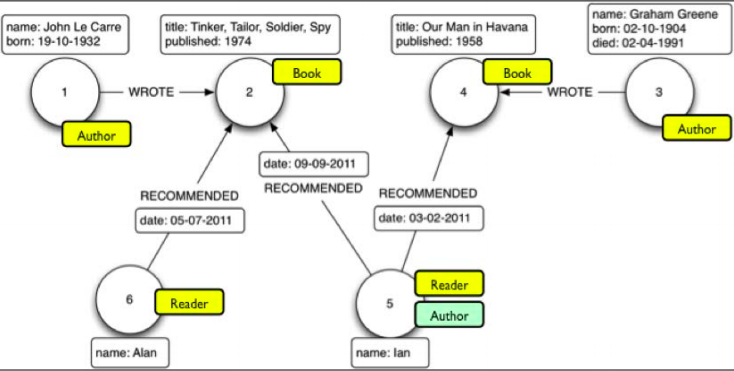
\includegraphics[scale=.60]{./Capitulo3/img/grafo-rotulado.png}
         \label{fig:propertygraphmodel}
     \fonte{Property Graph Model~\cite{bruggen:2014}}
 \end{figure}
 

•   Nodes: These are typically used to store entity information. In the preceding
example, these are the individual books, readers, and authors that are present
in the library data model.

•	 Relationships: These are used to connect nodes to one another explicitly
and therefore provide a means of structuring your entities. They are the
equivalent of an explicitly stored, and therefore pre-calculated, join-like
operation in a relational database management system. As we have seen
in the previous chapters, joins are no longer a query-time operation—they
are as simple as the traversal of a relationship connecting two nodes.
Relationships always have a type, a start- and an end-node, and a direction.
They can be self-referencing/looping and can never be dangling (missing
start- or end-node).

•	 Properties: Both nodes and relationships are containers for properties,
which are effectively name/value pairs. In the case of the nodes, this is
very intuitive. Just like a record in the relational database world has one or
more fields or attributes, so can the node have one or more properties. Less
intuitive is the fact that relationships can have properties too. These are used
to further qualify the strength or quality of a relationship and can be used
during queries/traversals to evaluate the patterns that we are looking for.

 Labels: This was a fundamental data model construct that was added to
Neo4j with Version 2.0 at the end of 2013. Labels are a means to quickly and
efficiently create subgraphs. By assigning labels to nodes, Neo4j makes the
data model of most users a lot simpler. There is no longer a need to work
with a type property on the nodes, or a need to connect nodes to definition
nodes that provide meta-information about the graph. Neo4j now does
this out of the box—and this is a huge asset, now and for the future. At
the time of writing this book, labels are primarily used for indexing and
some limited schema constraints. However, in future, it is likely that the
structural understanding that labels provide about the data stored in the
graph will be used for other purposes such as additional schema, security,
graph sharding/distribution—and perhaps others.


Uma das importantes funcionalidades do Neo4J é a utilização de plugins e bibliotecas para consulta ao banco de dados e execução de algoritmos de redes complexas. 
Dentre as várias bibliotecas podemos citar a \emph{Neo4j Graph Algorithms} que fornece um conjunto de procedimentos definidos pelo usuário que podem ser executadas através da linguagem de consulta Cypher.  
A biblioteca \emph{Neo4j Graph Algorithms} inclui algoritmos para análise de grafos e fluxos de trabalho de aprendizado de máquina com suporte a até dezenas de bilhões de nós e relacionamentos.

Outra biblioteca muito importante utilizada neste trabalho é a \emph{Neo4j Awesome Procedures on
Cypher (APOC)}. Esta biblioteca consiste em mais de 450 procedimentos e funções que auxiliam tarefas comuns como integração de dados, conversão de tipagem de dados e refatoração de modelos.


CYPHER

One of the defining features of the Neo4j graph database product today is its
wonderful query language, called Cypher. Cypher is a declarative, pattern-matching
query language that makes graph database management systems understandable and
workable for any database user—even the less technical ones.
The key characteristic of Cypher is, in my opinion, that it is a declarative language,
opposed to other imperative query languages that have existed for quite some time.

Why is this so important? Here are your answers:

•	 Declarative languages allow you to state what you're looking for, declare
the pattern that you would like to see retrieved, and then let the database
worry about how to go about retrieving that data.
In an imperative (query) language, you would have to tell the database
specifically what to do to get to the data and retrieve i


Declarative languages separate the concern of stating the problem, from
solving it. This allows greater readability of the queries that you write,
which is important as people tend to read their database queries more
often than they write them. This piece of your software will therefore
become more readable and shareable with others, and long term
maintenance of that easy-to-read query becomes so much easier.

•	 Declarative languages will allow the database to use the information that
it holds about the nature and structure of the data to answer your question
more efficiently. Essentially, it allows query optimizations that you would
never have known of or thought about in an imperative approach. Therefore,
declarative languages can be faster—at least over time as the optimization
algorithms mature.

•	 Declarative languages are great for adhoc querying of your database,
without you having to write complex software routines to do so.

\subsection{Apache Spark}


Apache Spark (doravante apenas Spark) é um mecanismo de análise para dados em grande escala pro‐
cessação. Ele usa uma abstração de tabela chamada DataFrame para representar e processar dados em
linhas de colunas nomeadas e digitadas. A plataforma integra diversas fontes de dados e
suporta linguagens como Scala, Python e R. Spark oferece suporte a várias análises
bibliotecas. Seu sistema baseado em memória opera usando gráficos de computação distribuídos de forma eficiente.

Apache Spark (henceforth just Spark) is an analytics engine for large-scale data pro‐
cessing. It uses a table abstraction called a DataFrame to represent and process data in
rows of named and typed columns. The platform integrates diverse data sources and
supports languages such as Scala, Python, and R. Spark supports various analytics
libraries, as shown in Figure 3-1. Its memory-based system operates by using efficiently distributed compute graphs.


\subsection{Transformação do \emph{dataset} para a base de dados de grafo do Neo4j}
\label{subsec:work}

A Figura~\ref{fig:workflow} mostra o fluxo de transformação dos dados para a construção do modelo de grafo no Neo4j a partir do \emph{dataset} disponibilizado. Diversos fluxos foram implementados na linguagem Python usando a ferramenta Apache Spark\footnote{https://spark.apache.org/}. 


 \begin{figure}[!h]
 \caption{Fluxo de ingestão de dados}
     \centering
     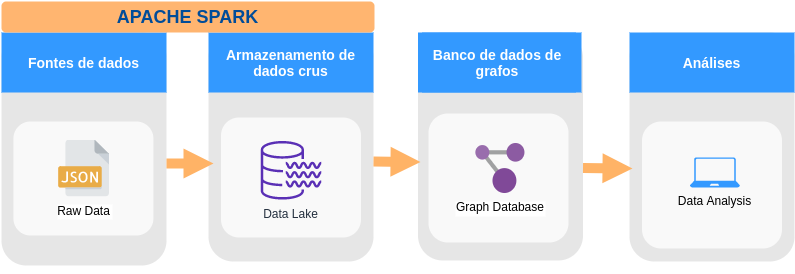
\includegraphics[scale=.45]{./Capitulo3/img/data-flow.png}
         \label{fig:dataflow}
     \fonte{Autoria própria}
 \end{figure}
 
 
A primeira etapa consiste no carregamento dos dados brutos (em formato JSON) para uma área temporária de armazenamento (ou \emph{data lake}). Os arquivos JSON são transformados em arquivos parquet\footnote{https://parquet.apache.org/} \cite{Boufea:17} utilizando o Apache Spark. Arquivos parquet são formatos de armazenamento em colunas, otimizados para compressão e rápida recuperação de dados. 
%Nesta etapa é realizada somente a transformação de formato de arquivo e armazenamento de dados em uma área denominada data lake.
Na sequência, o conteúdo do \emph{data lake} é processado - também usando o Apache Spark - para gerar arquivos no formato CSV com os vértices e arestas do modelo de grafo apresentado na Seção~\ref{sec:met}. 

Embora vários fluxos de transformação de dados tenham sido implementados, detalha-se a seguir as transformações dos dados que criam o vértice \emph{Stop} e a aresta \texttt{EVENT\_STOP} do grafo. Estas estruturas modelam a dinâmica de movimentação dos ônibus e justificam o uso de um grafo variante no tempo.
%\mar{(Keiko e Ricardo: mexi nessa linha. Veja se melhorou.}

% O vértice \emph{Stop} é criado a partir da tabela \emph{VEICULOS} (Tabela~\ref{tab:veiculos} do Apêndice), que contém a geolocalização dos ônibus nos respectivos instantes de tempo. Com essa informação, calcula-se a distância percorrida, o tempo decorrido entre posicionamentos consecutivos e a velocidade média em km/h. Se a velocidade for menor do que 15 km/h, assume-se que houve uma parada do ônibus neste intervalo de tempo e um vértice \emph{Stop} é gerado no grafo com os respectivos atributos.

O vértice \emph{Stop} é criado a partir dos dados de geolocalização dos ônibus nos respectivos instantes de tempo (ver descrição da tabela \emph{VEICULOS} no dicionário de dados do repositório). Com essa informação, calcula-se a distância percorrida, o tempo decorrido entre posicionamentos consecutivos e a velocidade média em km/h. Se a velocidade for menor do que 15 km/h, assume-se que houve uma parada do ônibus neste intervalo de tempo e um vértice \emph{Stop} é gerado no grafo com os respectivos atributos.

% A aresta \texttt{EVENT\_STOP} é criada a partir dos vértices \emph{Stop} previamente obtidos das linhas dos ônibus, dos pontos de ônibus e da tabela horária dos ônibus nas linhas (Tabelas~\ref{tab:linhas}, \ref{tab:pontos_linha} e \ref{tab:tabela_veiculo} do Apêndice, respectivamente). Se uma parada (vértice \emph{Stop}) ocorrer a menos de 20 m de um ponto de ônibus (vértice \emph{Bus Stop}), considera-se que tal parada ocorreu em um ponto de ônibus e, portanto, cria-se uma aresta \texttt{EVENT\_STOP} para conectar os vértices \emph{Stop} e \emph{Bus Stop} no grafo.
% Uma vez construído o banco de dados de grafo para o transporte, consultas e análises de redes complexas podem ser realizadas a partir do Neo4j (\emph{Data Analysis} na Figura~\ref{fig:workflow}).

A aresta \texttt{EVENT\_STOP} é criada a partir dos vértices \emph{Stop} previamente obtidos das linhas dos ônibus, dos pontos de ônibus e da tabela horária dos ônibus nas linhas (ver descrição das tabelas \emph{LINHAS}, \emph{PONTOS\_LINHA} e \emph{TABELA\_VEICULO}, respectivamente, no dicionário de dados do repositório). Se uma parada (vértice \emph{Stop}) ocorrer a menos de 20 m de um ponto de ônibus (vértice \emph{Bus Stop}), considera-se que tal parada ocorreu em um ponto de ônibus e, portanto, cria-se uma aresta \texttt{EVENT\_STOP} para conectar os vértices \emph{Stop} e \emph{Bus Stop} no grafo.
Uma vez construído o banco de dados de grafo para o transporte, consultas e análises de redes complexas podem ser realizadas a partir do Neo4j (\emph{Data Analysis} na Figura~\ref{fig:workflow}).
 
